\section{Scelta del modello}
Si riportano i valori di $R^2$, AIC e MSE dei cinque modelli.
\begin{table}[H]
	\centering
	\begin{tabular}{|c|c|c|c|}
		\hline
		\textbf{Modello} & \textbf{adjusted} \boldmath$R^2$ & \textbf{AIC} & \textbf{MSE}\\
		\hline
		1 &  0.77  & 514.69 & 155.54\\
		2 & 0.87 & 460.76 & 87.16\\
		3 & 0.89 & 448.27 & 61.72\\
		4 & 0.88 & 451.67 & 76.45\\
		5 & 0.91 & 431.91 & 55.65 \\
		\hline
	\end{tabular}
	\caption{Valori di $R^2$ e AIC per i quattro modelli}
\end{table}
\textbf{Osservazione.} È opportuno considerare che, nella scelta del modello, si è tenuto conto della discreta correlazione lineare osservata tra alcune variabili predittive, in particolare tra \textbf{x4\_MP} e \textbf{x7\_PixDensity} (correlazione pari a 0.743). \\ 
   Un’alta correlazione tra predittori può infatti dar luogo a fenomeni di \emph{multicollinearità}, ossia a situazioni in cui alcune variabili esplicative risultano linearmente dipendenti o quasi dipendenti. Ciò comporta una riduzione del rango della matrice di (\emph{design}), con conseguenti stime instabili dei coefficienti, varianze elevate e difficoltà nell’interpretazione individuale degli effetti delle singole variabili.
   
Di seguito vengono mostrati i grafici diagnostici ottenuti sui cinque modelli.
\begin{figure}[H]
	\centering
	\begin{minipage}{0.48\textwidth}
		\centering
		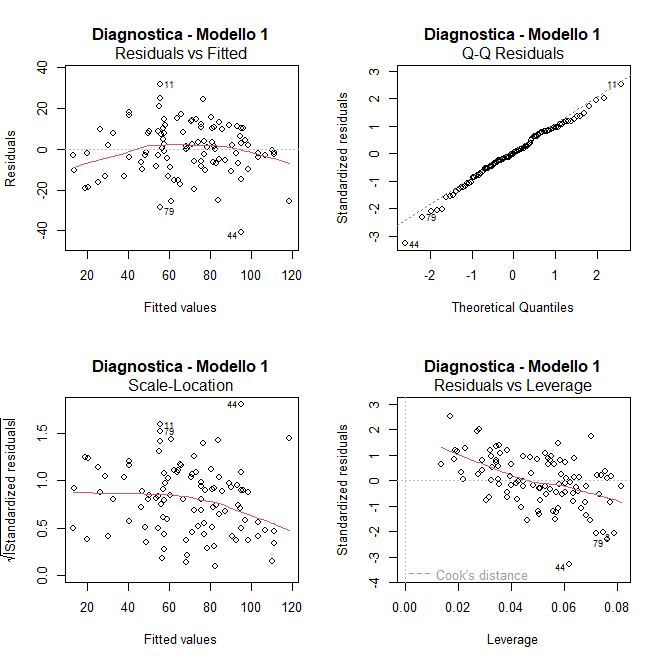
\includegraphics[width=\linewidth]{../graphs/diagnostica/modello1}
		\caption{Modello 1: diagnostica}
		\label{fig:diagnostica_modello1}
	\end{minipage}
	\hfill
	\begin{minipage}{0.48\textwidth}
		\centering
		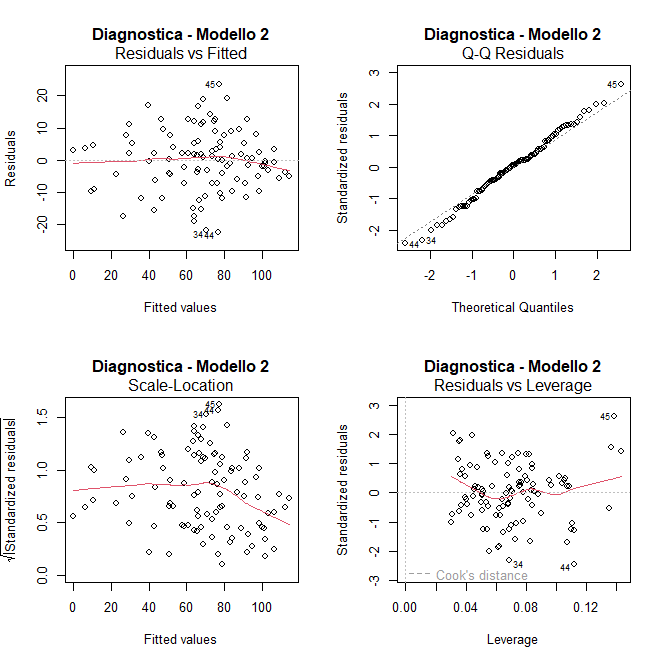
\includegraphics[width=\linewidth]{../graphs/diagnostica/modello2}
		\caption{Modello 2: diagnostica}
		\label{fig:diagnostica_modello2}
	\end{minipage}
\end{figure}

\begin{figure}[H]
	\centering
	\begin{minipage}{0.48\textwidth}
		\centering
		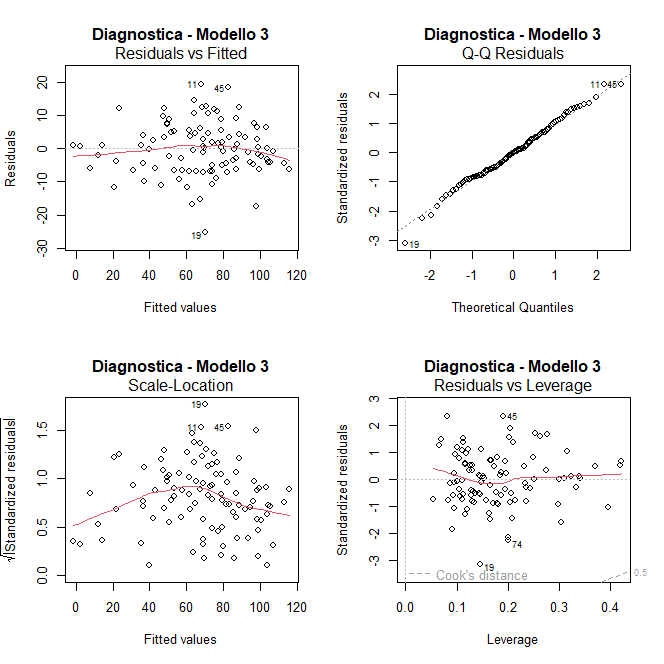
\includegraphics[width=\linewidth]{../graphs/diagnostica/modello3}
		\caption{Modello 3: diagnostica}
		\label{fig:diagnostica_modello3}
	\end{minipage}
	\hfill
	\begin{minipage}{0.48\textwidth}
		\centering
		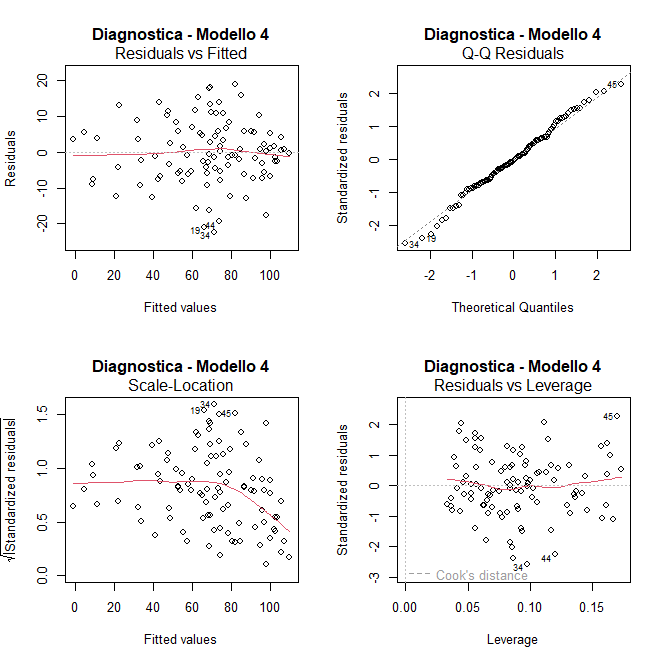
\includegraphics[width=\linewidth]{../graphs/diagnostica/modello4}
		\caption{Modello 4: diagnostica}
		\label{fig:diagnostica_modello4}
	\end{minipage}
\end{figure}

\begin{figure}[H]
	\centering
	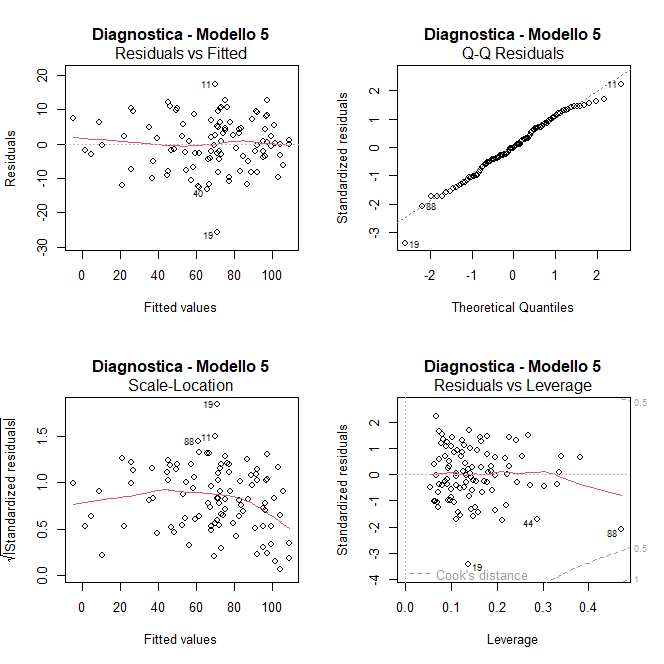
\includegraphics[width=0.75\linewidth]{../graphs/diagnostica/modello5}
	\caption{Modello 5: diagnostica}
	\label{fig:diagnostica_modello5}
\end{figure}

Osservando i grafici 'Residuals vs Fitted' si nota che nel modello 1, la linea rossa presenta un pattern, a differenza degli altri quat soddisfando in buona maniera l'ipotesi di linearità. Inoltre, sempre i modelli 2 e 4 nei grafici 'Q-Q Residuals' l'ipotesi di normalità sembra essere soddisfatta. 

Si osservi (dal grafico 'Scale-Location') che però su nessuno dei modelli considerati si può supporre che la varianza sia costante.

Infine comparando i valori di adjusted $R^2$ e AIC, il modello 4 sarebbe da preferire. Infatti, usando l'AIC, si sceglie il modello che ha valore minore; un valore maggiore di $R^2$ implica che il modello è in grado di interpretare meglio il fenomeno osservato.

A fronte dei dati ricavati si è stimato che il modello che meglio rappresenta il dataset fornito è il modello 4.


